\chapter{METODE PENELITIAN}

Bab ini memaparkan tentang metodologi penelitian yang digunakan pada penelitian ini.

\section{Solusi menggunakan repetisi kode biner}

Pada permasalahan pencarian Ulam non-interaktif, penjawab tidak diperbolehkan menjawab sebelum penanya selesai menanyakan seluruh query. Pendekatan pertama yang mungkin untuk menyelesaikan permasalahan ini adalah dengan mempersiapkan pencarian biner. Query awal pencarian biner berjumlah $q_b=log_2(n)$, agar setiap kemungkinan jawaban dari penjawab dapat mewakili semua kemungkinan nilai $x$. Lalu setiap query akan diulang sebanyak $q_e=2e+1$ kali agar penjawab pasti menjawab dengan jujur, karena $e$ query untuk jawaban bohong, ditambah dengan $e$ query untuk mengeliminasi jawaban bohong, ditambah dengan satu query jawaban pasti jujur karena kesempatan penjawab untuk berbohong sudah habis. Total jumlah query $q=q_b \times q_e$.

\begin{table}[h!]
\caption{Contoh pencarian biner pada $n=8$}
\label{tab:binary_8}
\begin{center}
\begin{tabu} {|X[l]|X[c]|X[c]|X[c]|X[c]|X[c]|X[c]|X[c]|X[c]|} 
\hline
$x$  & 1 & 2 & 3 & 4 & 5 & 6 & 7 & 8 \\
\hline
$Q_1$ & 0 & 0 & 0 & 0 & 1 & 1 & 1 & 1 \\
\hline
$Q_2$ & 0 & 0 & 1 & 1 & 0 & 0 & 1 & 1 \\
\hline
$Q_3$ & 0 & 1 & 0 & 1 & 0 & 1 & 0 & 1 \\
\hline
Jawaban & NNN & NNY & NYN & NYY & YNN & YNY & YYN & YYY \\
\hline
\end{tabu}
\end{center}
\end{table}

Misalnya jika $n=8$, $e=2$, $m=6$, maka jumlah $q_b$ untuk pencarian biner adalah 00001111, 00110011 dan 01010101 seperti pada Tabel \ref{tab:binary_8}. Dari tiga query, tersebut, semua jawaban penjawab mulai dari "NNN" sampai "YYY" dapat mewakili semua nilai $x$ dalam $S_n={1,2,...,8}$ sehingga nilai $q_b=3$. Lalu masing-masing query diulang sebanyak $q_e=2e+1=5$ kali. Maka total dari $q=q_b \times q_e=9$.


\section{Solusi menggunakan pembobotan Berlekamp}

Query pencarian biner dengan repetisi pasti dapat menyelesaikan permasalahan Ulam non-interaktif, namun jumlah query menghasilkan banyak redundansi. Oleh karena itu diperlukan pendekatan statistik peluang menggunakan pembobotan Berlekamp untuk mereduksi jumlah query. Gambar \ref{fig:flow_berlekamp} menjelaskan alur proses adalah membuat query pencarian biner terlebih dahulu, lalu dioptimasi menggunakan fungsi pembobotan berlekamp untuk menghitung peluang dari semua angka-angka dalam range $S_n$.

\begin{figure}
\centering
% 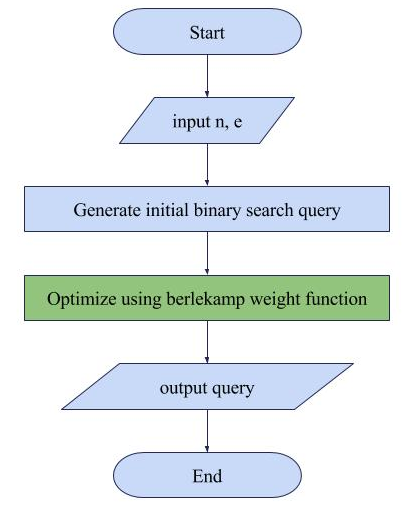
\includegraphics[scale=0.4]{../img/flowchart-berlekamp.png}
\begin{tikzpicture}[node distance=2cm]
% nodes
\node (start) [start] {Start};
\node (input) [io, below of=start] {Input n, e};
\node (proc1) [process, below of=input] {Generate initial binary search query};
\node (proc2) [process, below of=proc1] {Generate remaining query using Berlekamp function};
\node (output) [io, below of=proc2] {Output query};
\node (end) [start, below of=output] {End};
% draws
\draw[arrow]  (start) -- (input);
\draw[arrow]  (input) -- (proc1);
\draw[arrow]  (proc1) -- (proc2);
\draw[arrow]  (proc2) -- (output);
\draw[arrow]  (output) -- (end);
\end{tikzpicture}
\caption{Diagram alir solusi menggunakan pembobotan Berlekamp}
\label{fig:flow_berlekamp}
\end{figure}


\section{Solusi menggunakan kode biner}

Diberikan sebuah matriks $L$ berukuran $n \times M$ berisi $n$. Kumpulan query ini dinotasikan dengan $L = \{\vec{q_1},\vec{q_2},\ldots,\vec{q_n}\}$ dimana $\vec{q_i} = \{s_1,s_2,\ldots,s_M\}$. Himpunan nilai $s_i$ yang mungkin adalah $s_i \in \{0,1\}$. Diberikan sebuah vektor $\vec{z} \in \{z_1,z_2,\ldots,z_n\}$ dimana $z_i \in \{0,1\}$ berisi jawaban dari seluruh query secara berurutan, $z_i$ adalah jawaban dari $\vec{q_i}$, dimana $0$ berarti 'tidak' dan $1$ berarti 'ya'. Karena jika jawaban $0$ berarti query harus ditambah dengan 1 dan jika jawaban $1$ berarti query ditambah dengan 0 (diabaikan), maka kita memiliki $\vec{z'}$ yaitu inverse dari $\vec{z}$. 

Matriks $L'$ berukuran $M \times n$ adalah hasil transpose dari matriks $L$. Tambahkan seluruh baris pada $L'$ dengan $z'$. Maka jawaban dari permainan Ulam non-interaktif adalah index dari baris $r$ pada $L'$ yang memiliki bobot $wt(\vec{x_r}) > n-e$.

Penanya memenangkan permainan jika $L'$ memiliki paling banyak satu row dengan $wt(\vec{x}) \ge n-e$. Jika hanya ada satu row, maka row tersebut adalah jawaban permainan. Jika tidak ada satu row pun yang memenuhi, penanya tetap memenangkan permainan karena penjawab melakukan kecurangan, melakukan bohong untuk semua angka lebih dari batas yang ditetapkan.

Untuk meyakinkan bahwa setelah seluruh jawaban $\vec{z}$ diberikan dan diaplikasikan ke matrix $L$ dan tidak pasti hanya ada 1 baris yang memiliki nilai $1$ antara $n-e \le wt(\vec{x_r}) \le n$, adalah dengan memastikan bahwa jarak Hamming setiap row yang berbeda pada $L'$ adalah minimal $d$.

\begin{lemma}
Diketahui integer $n$, $M$, dan $d$. Jika $L'$ adalah kode biner $(n,M,d)_2$ yang valid, maka pasti hanya ada paling banyak satu codeword $\vec{c}$ yang memiliki $0 \le wt(\vec{c}) \le e$.
\end{lemma}

\begin{proof}
Jika ada codeword $c$ dimana $0 \le wt(c) \le e$ maka $wt(\vec{x}) > e$ dimana $\vec{x} \neq c$. Pembuktian dapat dibuktikan dengan dua kasus.\\

1) Jika $wt(\vec{c}) = 0$ maka
\begin{align*}
d_H(\vec{c},\vec{x}) &\ge d \mid \vec{c} \neq \vec{x} , \vec{x} \in L' \\
wt(\vec{c} + \vec{x}) &\ge d \\
wt(\vec{x}) &\ge d \label{eq:proofd} \stepcounter{equation} \tag{\theequation}
\end{align*}
Sebelumnya telah disebutkan hubungan $d$ dan $e$ pada \refeq{eq:de}. Persamaan tersebut dapat diturunkan menjadi
\begin{equation} \label{eq:dge}
d > e
\end{equation}
Dengan memasukkan \refeq{eq:dge} ke \refeq{eq:proofd}, maka didapatkan
\begin{equation*}
wt(\vec{x}) > e
\end{equation*}

2) Jika $wt(\vec{c}) = e$ maka
\begin{align*}
d_H(\vec{c},\vec{x}) &\ge d \mid \vec{c} \neq \vec{x} , \vec{x} \in L' \\
wt(\vec{c}+\vec{x}) &\ge d \\
wt(\vec{c}) + wt(\vec{x}) \ge wt(\vec{c}+\vec{x}) &\ge d \\
wt(\vec{c}) + wt(\vec{x}) &\ge d \\
e + wt(\vec{x}) &\ge d \\
\intertext{Masukkan \refeq{eq:de} untuk mensubstitusi $d$}\\
wt(\vec{x}) &\ge 2e+1-e \\
&\ge e+1\\
wt(\vec{x}) &> e
\end{align*}
Jadi jika ada codeword $c$ dimana $0 \le wt(c) \le e$ maka $wt(\vec{x}) > e$ dimana $\vec{x} \neq c$.
\end{proof}

Dari pembuktian diatas, dapat disimpulkan bahwa untuk menyelesaikan permainan pencarian Ulam non-interaktif dengan batas pencarian $M$ dan maksimal kebohongan $e$, transpose dari $n$ query yang dibuat harus membentuk kode biner $(n,M,d)_2$.

\begin{lemma}
Diketahui integer $n$, $M$, dan $d$. Jika $L'$ adalah kode biner $(n,M,d)_2$ yang valid, maka jika setiap codeword $\vec{c}$ pada $L'$ ditambah dengan $\vec{z} \mid \vec{z} \in \mathbb{F}_2^n$ maka hasilnya akan tetap menjadi kode biner $(n,M,d)_2$ yang valid.  
\end{lemma}

\begin{proof}
Jika $d_H(\vec{x_i},\vec{y_j}) \ge d \mid \vec{x_i},\vec{y_j} \in L'$ maka
\begin{align*}
d_H(\vec{x_i}+\vec{z},\vec{y_j}+\vec{z}) &\ge d \\
wt(\vec{x_i}+\vec{y_j}+\vec{z}+\vec{z}) &\ge d \\
wt(\vec{x_i}+\vec{y_j}) &\ge d \\
d_H(\vec{x_i},\vec{y_j}) &\ge d \\
\end{align*}
Jadi jika $d_H(\vec{x_i},\vec{y_j}) \ge d$ maka $d_H(\vec{x_i}+\vec{z},\vec{y_j}+\vec{z}) \ge d$.
\end{proof}
